\section{第一次迭代工作项管理}
\begin{frame}
    \frametitle{第一次迭代计划完成的用户故事}
    第一次迭代中,我们小组计划构建一个完整可用的软件系统架构,并且完成下列用户故事:
    \begin{figure}[H]
        \centering
        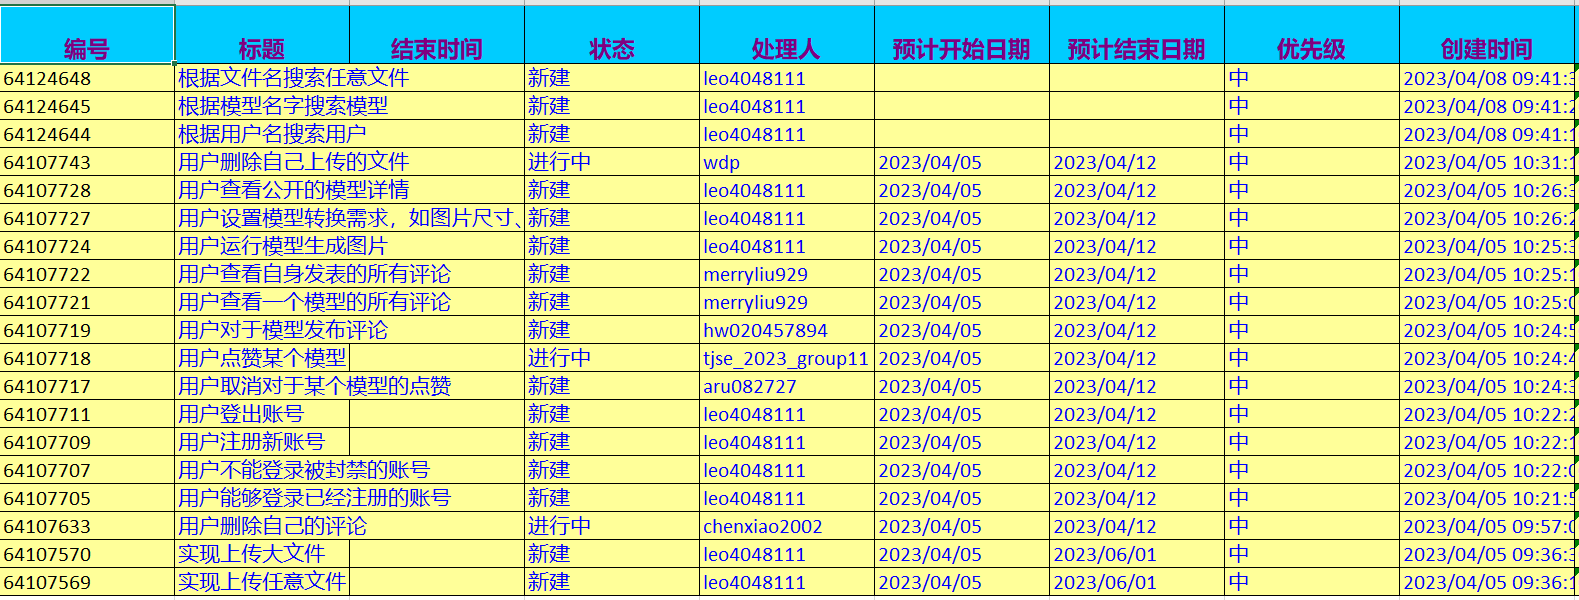
\includegraphics[width=\textwidth]{contents/figure/iteration1_stories.png}
    \end{figure}
\end{frame}

\begin{frame}
    \frametitle{第一次迭代软件系统功能测试项与测试结果}
    第一次迭代中,我们部署了Apifox项目,使用自动化工具结合手动测试的方式进行接责任划分管理、测试和文档生成,所有测试用例和结果已经登记到华为云平台,此处给出测试结果如下:
    \begin{figure}[H]
        \centering
        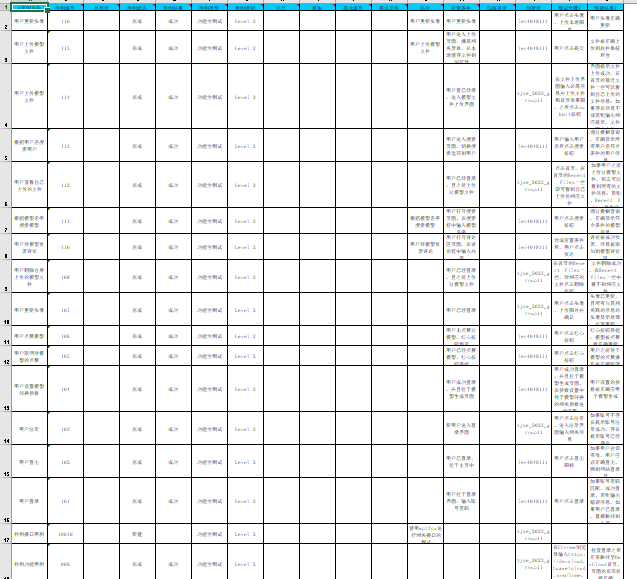
\includegraphics[width=\textwidth]{contents/figure/testcases.png}
    \end{figure}
\end{frame}

\begin{frame}
    \frametitle{燃尽图}
    \begin{figure}[H]
        \centering
        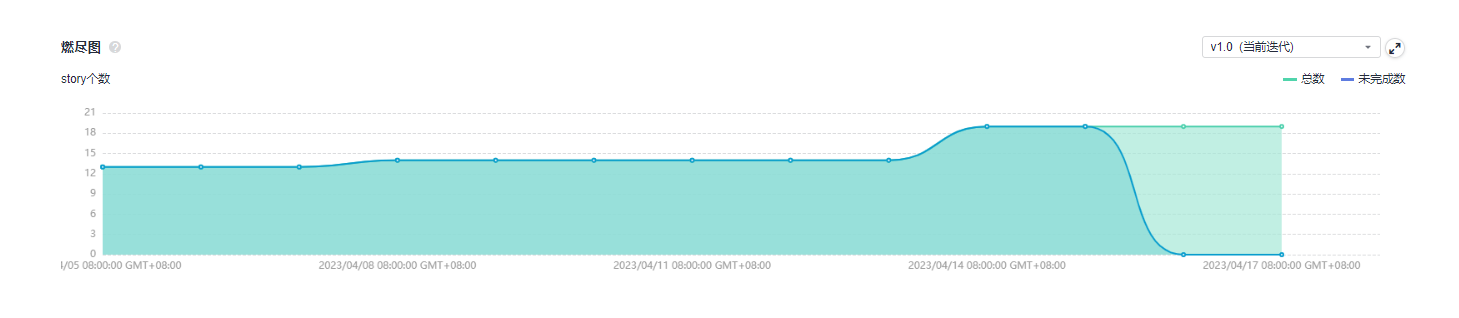
\includegraphics[width=\textwidth]{contents/figure/burnout.png}
    \end{figure}
\end{frame}

\begin{frame}
    \frametitle{量化贡献,按照组员负责的Story数和重要程度}
    \begin{figure}[H]
        \centering
        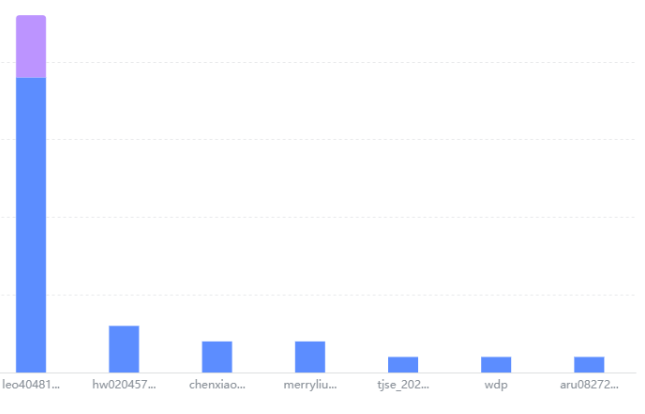
\includegraphics[width=0.8\textwidth]{contents/figure/contribution.png}
    \end{figure}
\end{frame}
